\section{Testing and evaluation}
\subsection{Overview}
A functional testing approach was taken as the main approach. 

A mock bank account management app has been setup using a simple Java web-server. The app was used for both testing and demonstration purposes.

A number of cases were implemented into the mock and expected the agent to handle:

\begin{itemize}
  \item Identify exceptions in other thread than the main one
  \item Identify exceptions driven by user input
  \item Deliver start/end and ping messages to the API
  \item Deliver exception logs to the API
  \item Correctly handle values of primitives and objects, statically and instance defined
  \item API engine unavailability
  \item Present a link to the Dashboard at the end of recorded stack-traces
\end{itemize}

\subsection{Agent testing and evaluation}
\subsubsection{Testing pipeline}
The main evaluation of the agent was done via the mock app. With each iteration of the agent, steps were taken to ensure this specific use-case was constantly fulfilled.

With every built attempt of the agent, if the built was successfully, the mock app would also be ran with the new agent attached.

\subsubsection{The mock Java bank account app}
The app uses a simple HttpServer setup, custom threads, timers and custom classes to assess and demonstrate the behaviour of the system

\begin{figure}[H]
  \centering
    
\includegraphics[width=\textwidth]{java-test.png}
  \caption[Mock bank account management app - Dashboard]{Mock bank account management app - Dashboard}
\end{figure}

\begin{figure}[H]
  \centering
    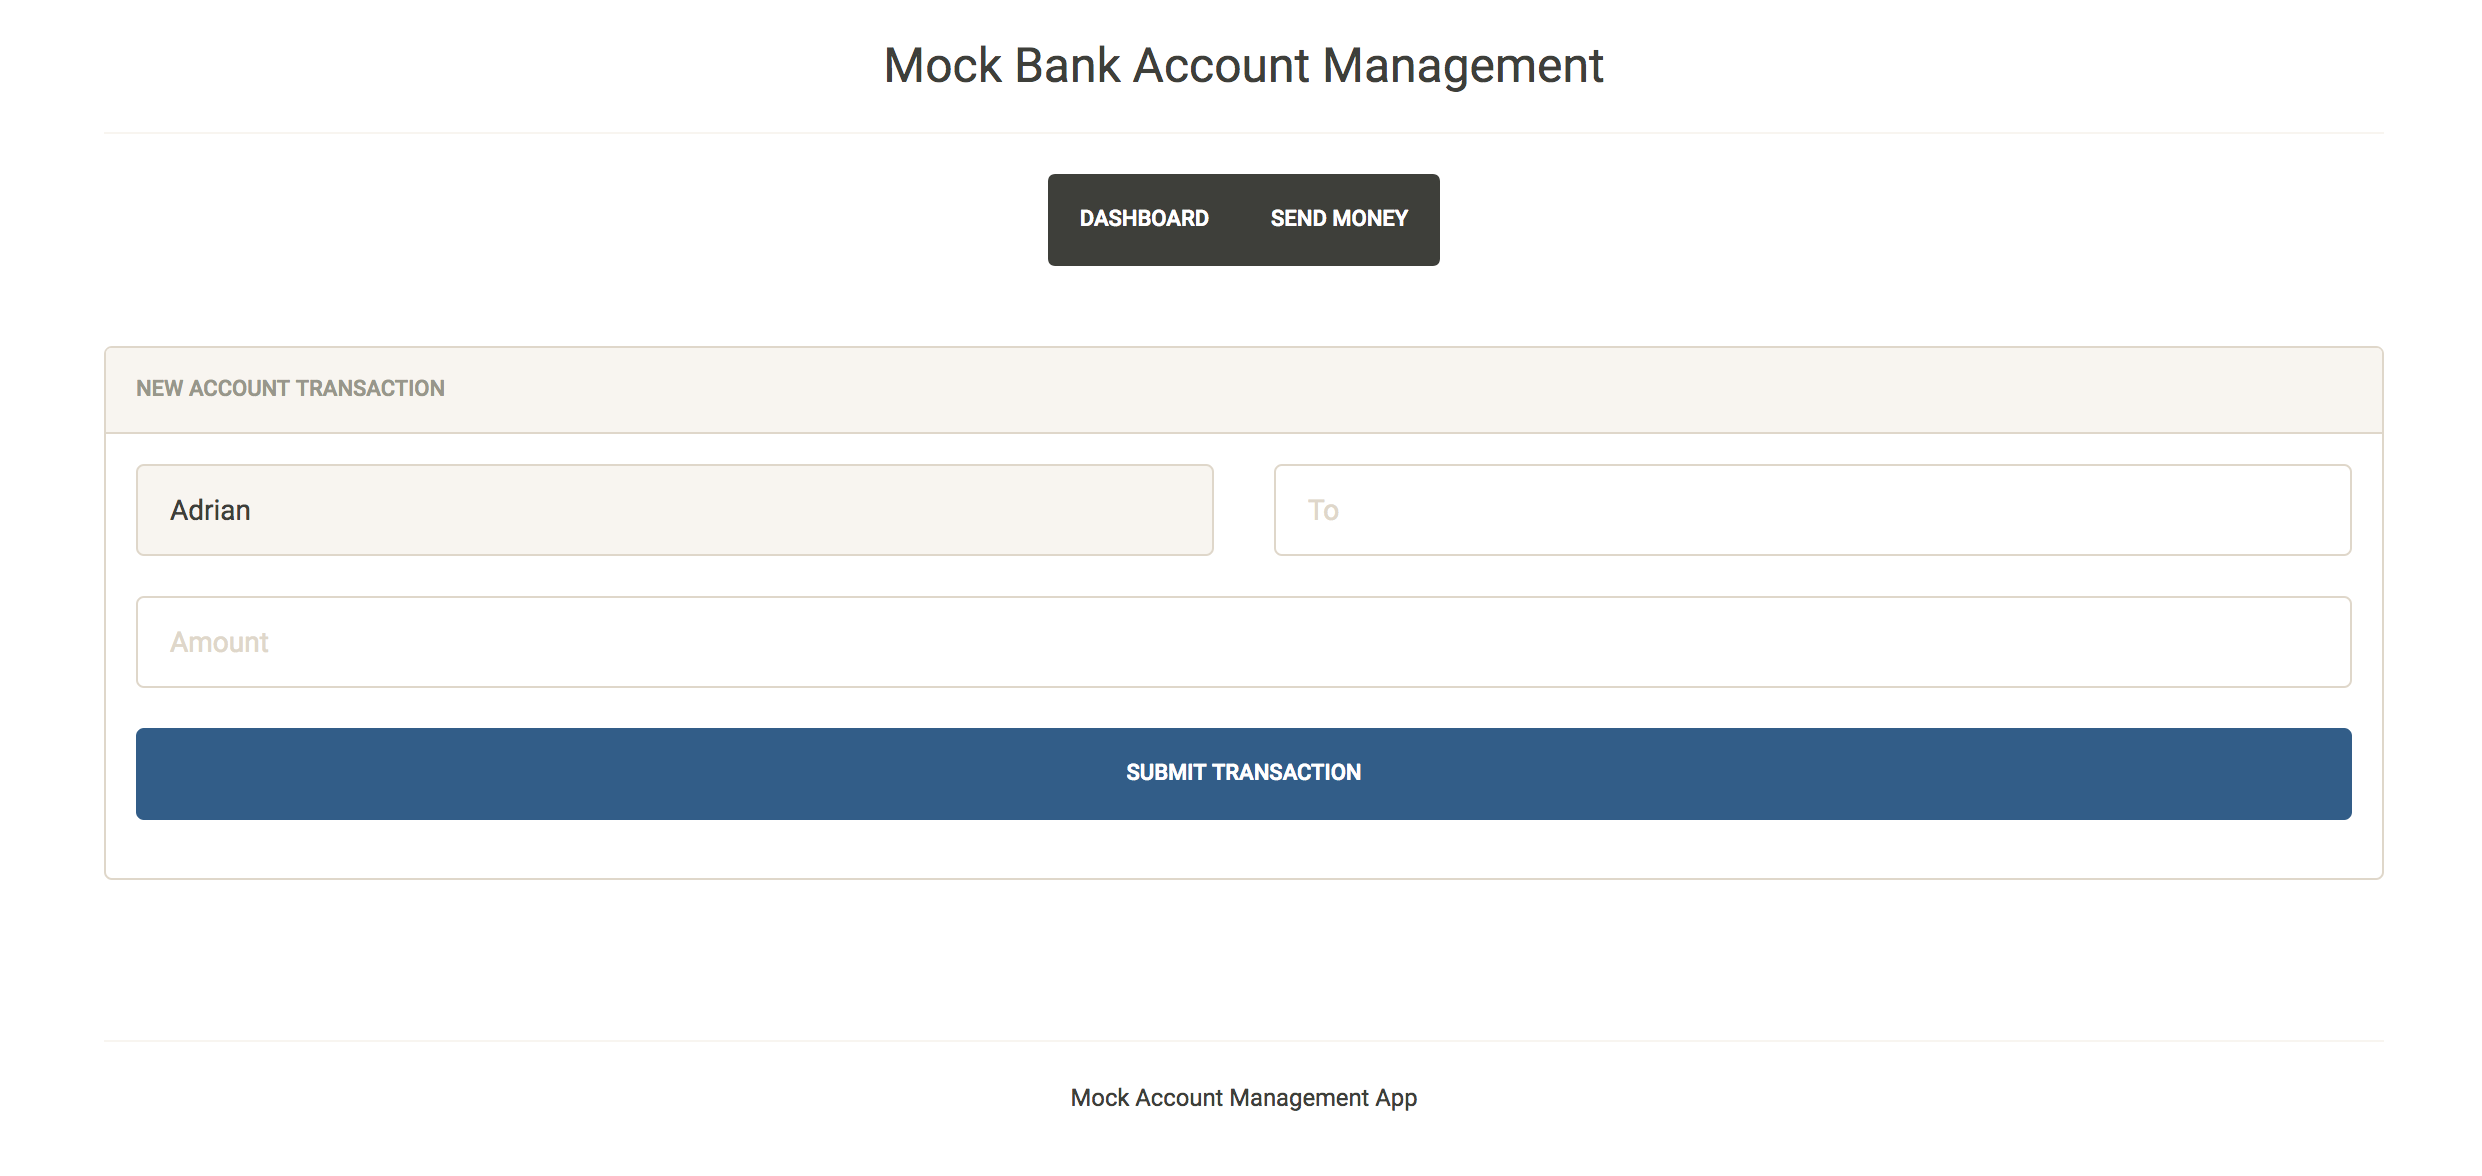
\includegraphics[width=\textwidth]{java-test2.png}
  \caption[Mock bank account management app - Submit transaction]{Mock bank account management app - Submit transaction}
\end{figure}

\begin{figure}[H]
  \centering
    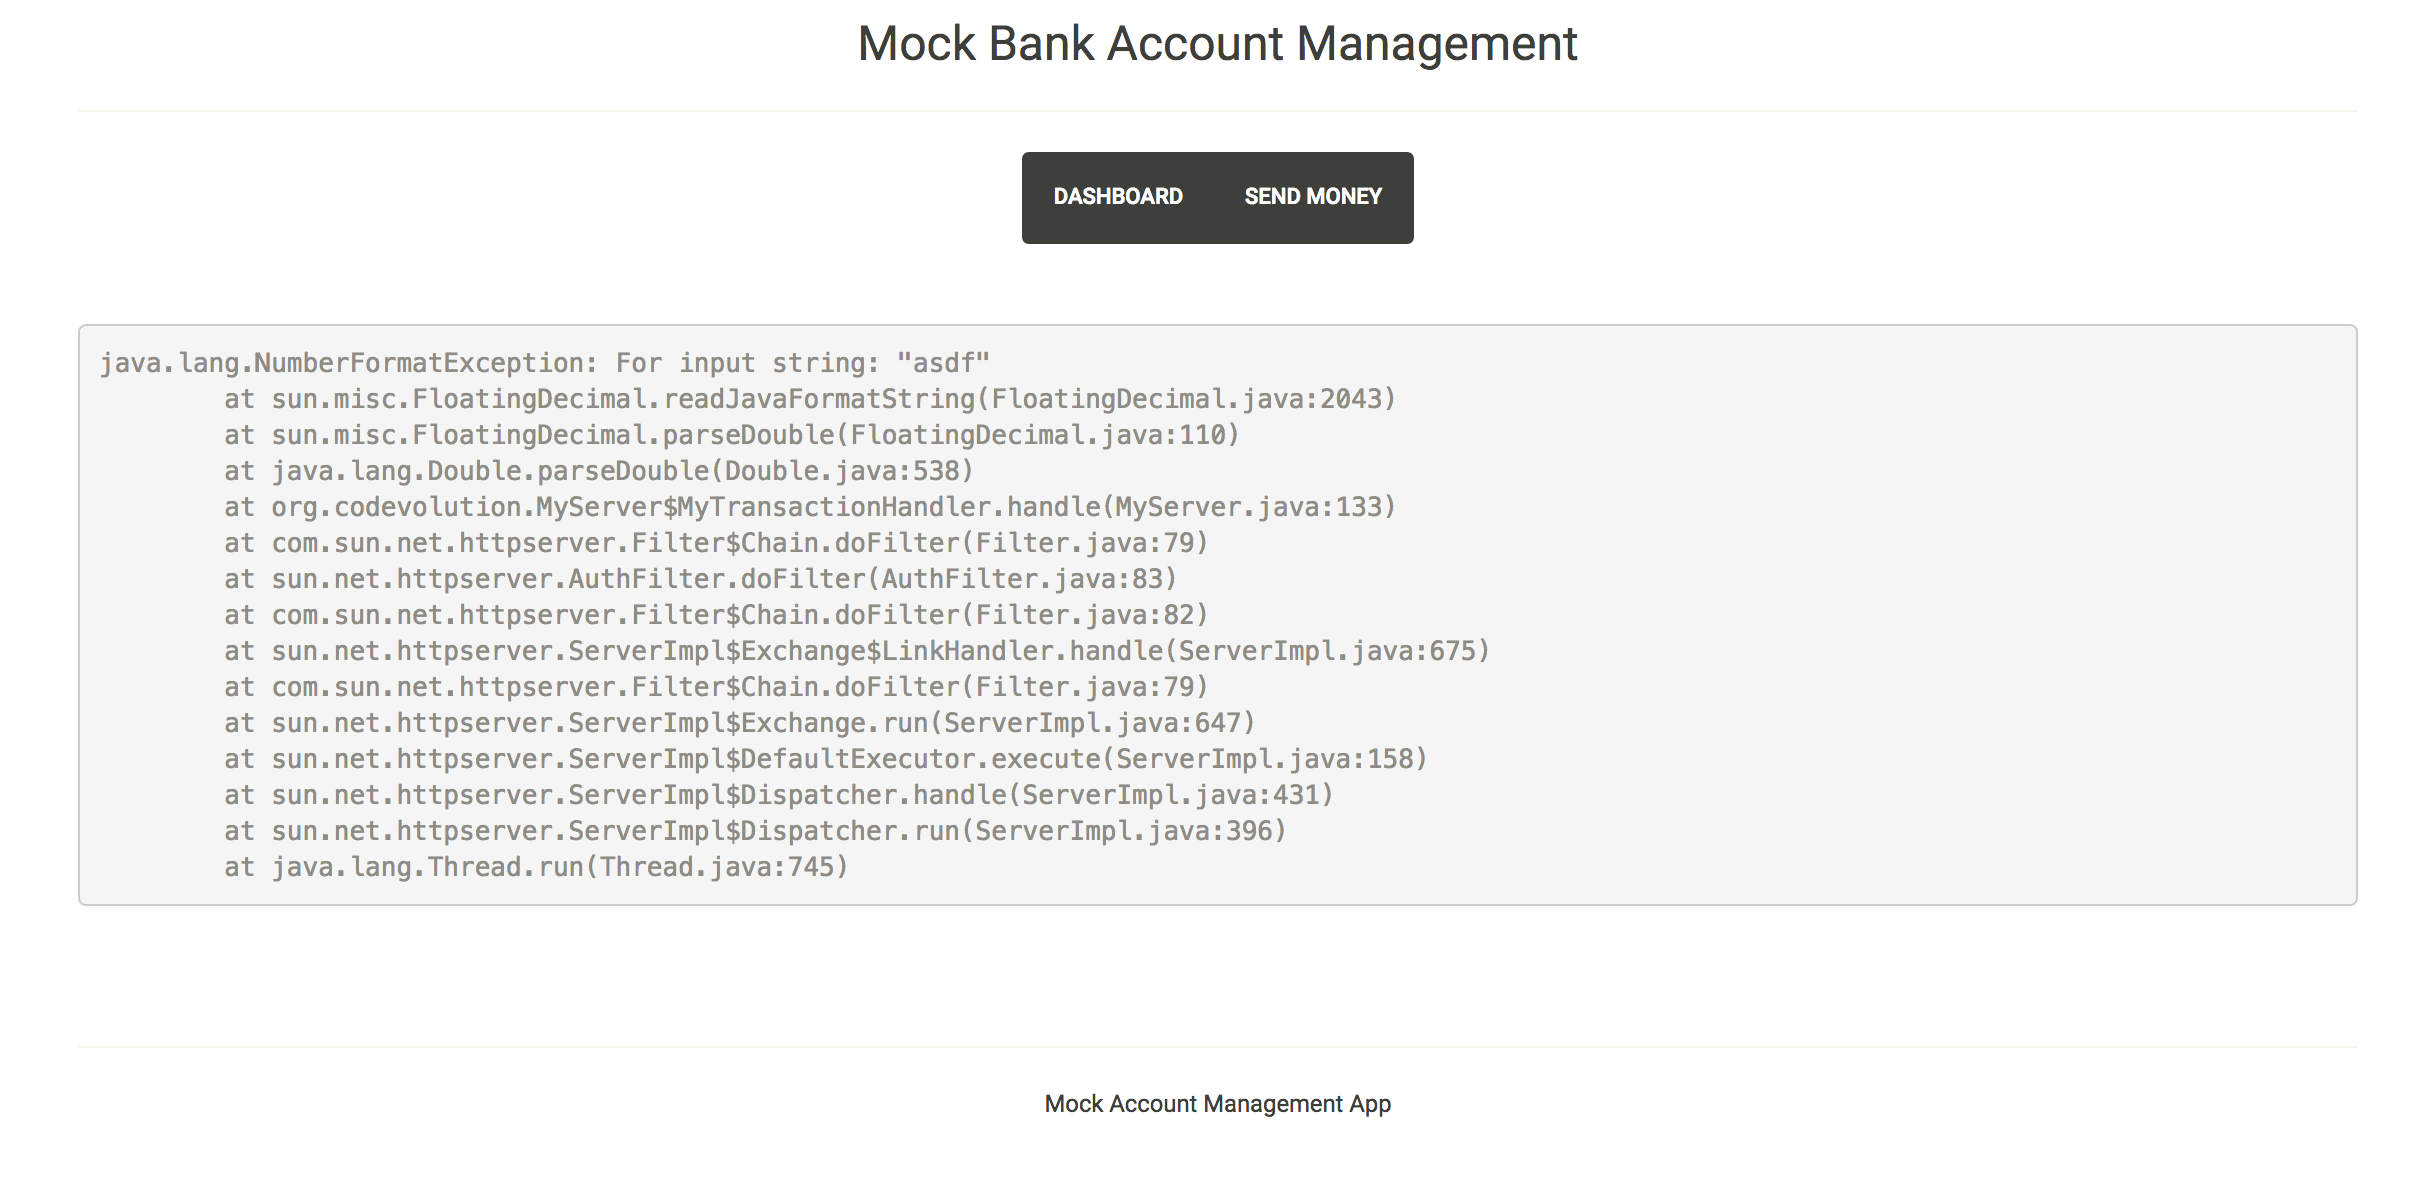
\includegraphics[width=\textwidth]{java-test3.png}
  \caption[Mock bank account management app - Exception]{Mock bank account management app - Exception}
\end{figure}

\subsection{Dashboard testing and evaluation}
This proved to be one of the most difficult parts to test as external testers would needs their agent to communicate to a server were an instance of the API engine would be running and one of the Dashboard.

Three students contributed by using the agent on their personal JVM-based apps and then employing the use of the dashboard to analyse the results.

An Amazon Web Service instance of the API engine and Dashboard were setup for this purpose and their use of the agent was done in both controlled  and uncontrolled environments.

\subsection{Operating systems}
The system was mostly tested using macOS Sierra driven machines with limited Windows testing.

The API engine was ran on macOS Sierra and Ubuntu 16 machines.

\subsection{Concluding remarks}
Given all the different components of the system, it proved hard to have all-around testing, especially due to the operating-system specific builds required for the agent component.

Moreover, finding external test users was challenging due to the technical learning curve needed to use the agent and the high level of system reliability required even for basic usage.


\newpage